% vim: spelllang=es

\chapter{Implementación}

\section{Metodología}

\newcommand{\work}{``Primero que Funcione''\xspace}

Antes de nada, es importante aprender un poco sobre cómo realizar cambios en el
código de Tremor eficientemente. Este proyecto modificará gran cantidad de
líneas y cuanto más rápido sea el desarrollo, menos problemas habrán. Esto se
puede cubrir de forma específica al lenguaje Rust, con trucos o consejos que
puedan facilitar el desarrollo, o de forma más general, con la estrategia de
trabajo a seguir. En esta sección se cubrirá lo último, dado que es menos un
detalle de implementación.

TODO: podría mencionar trucos relacionados con Rust en detalle (desactivar
algunos warnings, o quitar statements \code{use}), pero no creo que sea tan
importante en este caso y el documento ya es bastante largo.

La metodología fue insipirada por mis mentores, que lo denominaron el ``Just
Make it Work'', o \work. Se basa en que, inicialmente, con lo que más problemas
tenía era el perderme en los detalles. Pero ciertamente, primero de todo lo
importante es que ``funcione''. Siempre y cuando el sistema de plugins se pueda
compilar y ejecutar, lo siguiente es secundario:

TODO: alguna traducción de "just make it work" un poco más natural? "Solo que
funcione"? "No te líes, que funcione primero"?

\begin{itemize}
    \item Código ``feo'' (no idiomático, repetitivo o desordenado).

    \item Código de bajo rendimiento.

    \item Documentación pobre.

    \item No tener tests.

    \item No aplicar sugerencias recomendadas por \emph{linters} (en el caso de
        Rust, \emph{Clippy}).

\end{itemize}

TODO: el siguiente párrafo puede no gustarle a alguno de ingeniería del software
porque rompe todas las metodologías de desarrollo que tienen, pero fue como
sinceramente ocurrió.

El no trabajar con tests es discutible, dado que depende de si el programador
prefiere seguir un desarrollo basado en tests. Sin embargo, personalmente no
sentí la necesidad de escribir ningún test en este caso, al menos al principio.
Gracias al sistema fuertemente tipado de Rust, fue principalmente un
\emph{desarrollo basado en el compilador}. Mi progreso se basaba en realizar
algunos cambios y posteriormente intentar que los aceptara el compilador,
repetidamente. Únicamente avancé a la parte de tests cuando todo parecía
funcionar manualmente y estaba lo suficientemente satisfecho con el resultado.

Adicionalmente, las optimizaciones prematuras son la fuente de todos los
problemas. No es algo que sea importante aún. Solo una vez terminada la primera
iteración se puede dedicar más tiempo a medir el rendimiento para saber cuáles
optimizaciones merecen la pena. Notar que sí es importante escoger un
\emph{método o tecnología} que sea apropiado en términos de rendimiento; fue por
ello por lo que se descartó WebAssembly o IPC en el capítulo anterior. Pero
definitivamente el desarrollador debería rendirse en, por ejemplo, evitar una
conversión entre dos tipos innecesaria que posiblemente no afecte al rendimiento
al fin y al cabo.

Lo que quería dejar claro el equipo de Tremor es que todos los tests, limpiezas
u optimizaciones que intentes realizar en este momento acabará muy probablemente
siendo en vano. Se llegará a un punto en el que no se pueda continuar y que
requiera repensar y reescribir gran parte del trabajo. Cuando todo compile y
aparentemente funcione correctamente, se puede dedicar esfuerzo a trabajar en
estos temas secundarios. Si algo no importante está llevando demasiado tiempo,
se debería marcar como TODO o FIXME y dejarlo para otro momento.

Notar que no hay problema con ``gastar'' el tiempo con métodos que acaban siendo
incorrectos, porque realmente no se está ``gastando'' nada; son un paso
necesario para llegar a la solución final. Pero es doloroso tener que eliminar
código al que le has dedicado tiempo, así que al menos debería intentarse
minimizar el impacto que esto tenga.

\section{\abistable}

Dado que \abistable va a ser la librería principal en la que se basará el
sistema de plugins, es importante entender cómo funciona al completo. Además de
conocer los detalles de implementación, es importante conocer cómo \abistable
soluciona los problemas a tener en cuenta para implementar un sistema de
plugins:

\subsection{Versionado}

\abistable especifica lo siguiente respecto a su sistema de
seguridad~\cite{abistable_safety}:

\begin{itemize}
    \item El ABI de \abistable se comprueba siempre. Cada versión \code{0.y.0} y
        \code{x.0.0} de \abistable define su propio ABI, que es incompatible
        con versiones anteriores.

    \item Los tipos se comprueban recursivamente cuando se carga una librería
        dinámica, antes de llamar ninguna función.

\end{itemize}

Todo esto se basa en el \trait \code{StableAbi}, indicador de que un tipo es
seguro para FFI. Contiene información sobre la estructura en memoria y puede ser
derivado automáticamente. Todos los tipos exportados por \abistable, además de
usar el ABI de C, implementan dicho \trait. Por tanto, si queremos declarar
nuestro propio tipo para usar con \abistable, ademaś de marcarlo con
\code{#[repr(C)]}, tendremos que añadir \code{#[derive(StableAbi)]}.

\subsection{Cargado de plugins}

\subsection{Exportando un plugin}

\subsection{Gestión de pánicos}

Actualmente, lanzar pánicos a través del FFI es comportamiento no
definido~\cite{panicsnomicon}. Aunque el programa aborte en la mayoría de los
casos, no existe ninguna garantía de que vaya a suceder así; podría continuar en
un estado inválido, con cualquier tipo de consecuencia.

La solución más directa es usar la función \code{std::panic::catch_unwind}, que,
para casos excepcionales como este, puede parar la propagación de pánicos cuando
sea llamada. Se podría usar en todas las funciones exportadas por el plugin
internamente, y en caso de producirse un pánico se abortaría el programa, en
lugar de dejar que se propague a la runtime, que sería indefinido.

También es posible configurar el programa para que aborte cuando se produzca un
pánico, en vez de propagarlo. De esta forma, no se llegaría a invocar
comportamiento no definido y se mantendría un rendimiento máximo --- capturar
pánicos tiene un coste. Sin embargo, implica varias desventajas importantes: al
abortar, no se tendrá acceso a la información de \emph{debug} que dan los
pánicos, tampoco se limpiará el estado del programa, y desde la runtime es
imposible saber si el plugin ha configurado los pánicos para que aborten. Esto
último será posible en el futuro, una vez \textcite{pluggablepanic} llegue a una
versión estable.

Esto es algo que \abistable ha tenido en cuenta desde el principio. Antes de que
un pánico se vaya a propagar de plugin a runtime, la librería abortará el
programa por completo. Esta parte se realiza de forma transparente; no hace
falta que el desarrollador se preocupe en ningún momento por ello.

La solución de \abistable no es perfecta por tener un pequeño coste de
rendimiento y por imposibilitar el recuperarse de errores en los plugins. En una
futura versión de Tremor, podría ser posible reiniciar plugins en caso de que
dejen de funcionar para mejorar la resiliencia a fallos.

El equipo de Rust conoce esta limitación y está trabajando en mejorar la
situación. En una futura versión, planea definir cuándo se puede propagar un
pánico de forma más precisa~\cite{cunwind}.

\subsection{Programación asíncrona}

El objetivo inicial era simplificar la interfaz lo suficiente como para que no
sea necesario tratar aspectos como programación asíncrona en el PDK. Esto
terminó siendo inevitable, dado que la asincronía es uno de los pilares de
Tremor.

TODO: podría poner un ejemplo de cómo se usa esta librería (está en un
comentario aquí), pero creo que es demasiado detalle.

% \begin{minted}{rust}
% // Así funciona la programación asíncrona en Rust; la primera
% // función es prácticamente equivalente a la segunda.
% async fn example() -> String {
%     read_file().await
% }
% fn example() -> impl Future<Output = String> {
%     async {
%         read_file().await
%     }
% }
%
% // No pueden haber genéricos en FFI, por lo que ahora `Future`
% // es un tipo concreto `FfiFuture` en vez de un trait. La
% // conversión de `Future` a `FfiFuture` se puede realizar con
% // `into_ffi`.
% fn example() -> FfiFuture<String> {
%     async move {
%         read_file().await
%     }
%     .into_ffi()
% }
% // `FfiFuture<T>` implementa `Future<Output = T>`, por lo que
% // su uso es el mismo.
% async fn user() {
%     example().await
% }
% \end{minted}

Para poder usar \code{async} con el ABI de C se puede recurrir a la \crate
\cratelink{async_ffi}, cuyo único problema era no tener soporte para \abistable.
Al no implementar el \trait \code{StableAbi}, no se podía usar en la interfaz
del PDK, por lo que tuve que abrir un pull request para hacerlo yo
mismo~\cite{asyncfficontrib}. El uso de esta librería resulta en código más
verboso, pero esto se podría mejorar en el futuro con un macro
procedural~\cite{asyncffimacro}.

\subsection{Seguridad en hilos}

\abistable utiliza la \crate \cratelink{libloading} internamente, cuya gestión
de errores no es segura en hilos en algunas plataformas, como \code{dlerror} en
FreeBSD~\cite{thsafe_libloading}\cite{thsafe_openbsd}. Sí que lo es en
Linux~\cite{thsafe_linux}, macOS~\cite{thsafe_macos} y Windows~\cite{thsafe_ms},
así que en el caso de Tremor no hace falta preocuparse por esto.

Será importante tener esto en cuenta en el futuro; al añadir soporte para un
nuevo sistema operativo habrá que asegurarse de que su gestión de errores sea
segura en hilos. En caso contrario, deberá actualizarse \code{libloading} para
sincronizar el acceso con un mútex interno, como lo hace la \crate
\cratelink{dlopen}~\cite{thsafe_dlopen}. Notar que esta librería es también
mejorable, dado que usa el mútex siempre, incluso en sistemas operativos donde
el sistema de errores sí es seguro en hilos~\cite{thsafe_dlopen_issue}.

\subsection{Rendimiento}\label{abiperf}

Un último punto vital a tener en cuenta es el coste de realizar conversiones
entre tipos de la librería estándar y tipos de \abistable. Esto se dará en
numerosas ocasiones, dado que usar \abistable cuando no es necesario es
subóptimo para tanto el rendimiento como la usabilidad. Y si, por ejemplo,
convertir un \code{Vec<T>} a un \code{RVec<T>} tuviese complejidad $O(n)$,
probablemente \abistable tendría que ser descartado como la solución escogida.

Afortunadamente, tras analizar la implementación de tipos como \code{RVec<T>},
\code{RSlice<T>}, \code{RStr} o \code{RString}, estas conversiones únicamente
consisten en transferir un puntero con los datos, sin necesidad de copiar nada.
Es decir, las conversiones que realizaremos serán $O(1)$.

\section{Conversión al ABI de C}

El primer paso en el proceso es declarar toda la interfaz del PDK de forma que
use el ABI de C, en vez del de Rust. Esto se puede hacer con el atributo
\code{#[repr(C)]} (en lugar del \code{#[repr(Rust)]} implícito), pero el
problema reside en que todos los tipos dentro suyo \emph{también} tendrán que
haber sido declarados con dicho atributo. Para ilustrarlo mejor, la estructura
más complicada al respecto fue \code{Value}, usado para representar datos
pseudo-JSON y definido a continuación de forma simplificada:

\begin{minted}{rust}
pub enum Value {
    /// Valores estáticos (enteros, booleanos, etc)
    Static(StaticNode),
    /// Tipo para cadenas de caracteres
    String(String),
    /// Tipo para listas
    Array(Vec<Value>),
    /// Tipo para objetos (mapas clave-valor)
    Object(Box<HashMap<String, Value>>),
    /// Tipo para datos binarios
    Bytes(Vec<u8>),
}
\end{minted}

Para poder usar \code{Value} en la interfaz del sistema de plugins, se puede
convertir a:

\begin{minted}{rust}
#[repr(C)] // La representación en memoria de Value seguirá el ABI de C
#[derive(StableAbi)] // Solo necesario cuando se usa abi_stable
pub enum Value {
    Static(StaticNode),
    /// Ahora usa `RString`, la altenativa a `String` de abi_stable
    String(RString),
    /// De forma similar, usa `RVec` en vez de `Vec`
    Array(RVec<Value>),
    /// Cambio de `Box`, `HashMap` y `String` por sus alternativas
    Object(RBox<RHashMap<RString, Value>>),
    /// Otro cambio de `Vec`
    Bytes(RVec<u8>),
}
\end{minted}

El primer problema surge en la variante \code{Static}. Su tipo contenido
internamente, \code{StaticNode}, es externo y usa \code{#[repr(Rust)]}. Se
declara en el \crate \cratelink{value_trait}, que lo declara tal que:

\begin{minted}{rust}
pub enum StaticNode {
    I64(i64),
    U64(u64),
    F64(f64),
    Bool(bool),
    Null,
}
\end{minted}

Esto se podría arreglar siguiendo el mismo procedimiento recursivamente, hasta
que todo sea \code{#[repr(C)]}. Pero como se trata de una librería externa,
tendrá que abrirse un nuevo pull request y esperar que al autor le parezcan bien
los cambios~\cite{openstaticnode}. Será importante también que la estructura use
\code{#[repr(C)]} únicamente cuando opcionalmente se configure a tiempo de
compilación como necesario. De esta forma, el resto de usuarios podrán seguir
aprovechándose de las ventajas de rendimiento que ofrece \code{#[repr(Rust)]}.

\subsection{Consecuencias del sistema de plugins}

Por desgracia, este cambio no termina ahí; cambiar las variantes de \code{Value}
implica que el código que lo usaba se romperá de numerosas formas:

\begin{minted}{rust}
// No funcionará porque Value::Array contiene un RVec ahora
let value = Value::Array(Vec::new());
\end{minted}

Este caso es el más sencillo: simplemente hace falta cambiar \code{Vec} por
\code{RVec}. La intención de los tipos de \abistable es que sean un reemplazo
directo de los de la librería estándar, i.e., su interfaz será la misma:

\begin{minted}{rust}
let value = Value::Array(RVec::new());
\end{minted}

% TODO: 'return' es devolver o retornar?
Es un poco más complicado cuando los tipos anteriores se exponían en métodos,
porque requiere tomar una decisión entre expandir el límite de FFI del
\emph{funcionamiento interno} de \code{Value} a los \emph{usuarios} de
\code{Value}. Por ejemplo, la variante \code{Value::Object} contiene un
\code{RHashMap} ahora, pero el método \code{Value::as_object} solía devolver una
referencia a \code{HashMap}. Se producirá un error nuevo ahí y tendrá que
tomarse la decisión de devolver \code{RHashMap} o añadir una conversión interna
a \code{HashMap}:

\begin{minted}{rust}
impl Value {
    // Código original
    fn as_object(&self) -> Option<&HashMap<String, Value>> {
        match self {
            // Problema: `m` ahora es una `RHashMap`, pero la función
            // devuelve un `HashMap`.
            //
            // Solución 1: cambiar el tipo devuelto a `RHashMap`
            // Solución 2: convertir `m` a un `HashMap` con `m.into()`
            Self::Object(m) => Some(m),
            _ => None,
        }
    }
}
\end{minted}

\begin{itemize}
    \item Si se cambia el tipo devuelto a \code{RHashMap}, casi todas las veces
        que se llamaba a \code{as_object} ahora dejarán de compilar porque se
        esperan un \code{HashMap}.

        Esto puede ser complicado porque, para evitar realizar conversiones, el
        sistema de plugins \emph{infectaría} la base de código por completo.
        Tendría que propagarse el uso de \code{RHashMap} por todo el programa,
        incluso cuando el PDK no es importante. Por ejemplo, \code{Value}
        también se usaba en la implementación del lenguaje de Tremor, Troy.
        Tener que usar un \code{RHashMap} en esa situación sería confuso y
        acabarían modificándose gran cantidad de ficheros sin relación al
        sistema de plugins.

    \item Si se realiza una conversión interna a \code{HashMap} en
        \code{as_object}, evitaremos todos esos errores, con un pequeño coste de
        rendimiento. Es la opción más fácil, pero si \code{Value::as_object} se
        usara frecuentemente, e.g., en el bucle principal, sí que podría causar
        una degradación considerable.
\end{itemize}

Como indica la sección~\ref{abiperf}, las conversiones entre la librería
estándar y \abistable son $O(1)$. Esto es dónde la metodología \work es
relevante: simplemente dejaremos el límite del FFI en su mínimo y añadiremos
conversiones cuanto antes sea posible. Al terminar, si se detectan problemas de
rendimiento en un caso en concreto, se puede reconsiderar.

\subsection{Problemas con tipos externos}

En algunos casos, los tipos de \abistable no habían sido actualizados para
incluir métodos nuevos de la librería estándar, por lo que era necesario un pull
request para añadirlo\footnote{El anexo \ref{annex:contributions} lista todas
las contribuciones de código abierto realizadas para este proyecto}. Pero por lo
general, convertir los tipos \emph{de la librería a estándar a \abistable} es
una tarea trivial, simplemente un tanto tedioso.

Los problemas surgen cuando es necesario convertir \emph{tipos externos a
\abistable}. La declaración anterior de \code{Value} era una simplificación;
realmente, Tremor usa la implementación de \cratelink{halfbrown} de
\code{HashMap<K, V>}. Esto se debe a que es más eficiente para su caso de uso, y
que posee algunas funcionalidades adicionales necesarias. El mismo caso se da
para otro tipo \code{Cow}, cuya alternativa en la \crate \cratelink{beef} ocupa
menos espacio en memoria y ofrece un mejor rendimiento en Tremor.

Ninguno de estos dos tipos tienen soporte dentro de \abistable, y aunque estos
tipos estén basados en otros de la librería estándar, la conversión no es
directa. Se pueden tomar cuatro posibles alternativas:

\subsubsection{Evitar el tipo externo}

Basándose en \work, una solución perfectamente válida es eliminar las
optimizaciones temporalmente y dejar un \code{TODO} para que se pueda revisar
posteriormente. Es posible que el sistema de plugins tenga excesiva complejidad,
y limitarse a usar tipos de la librería estándar podría ser suficiente.

En el caso específico de \code{Value}, eliminar las optimizaciones problemáticas
parece la manera más fácil de arreglar el problema. Y lo sería, si no fuera
porque eliminar código también puede ser complicado, como muestra la
Figura~\ref{fig:errors}, especialmente cuando la funcionalidad extra del tipo
externo no está disponible.

\begin{figure}
    \centering
    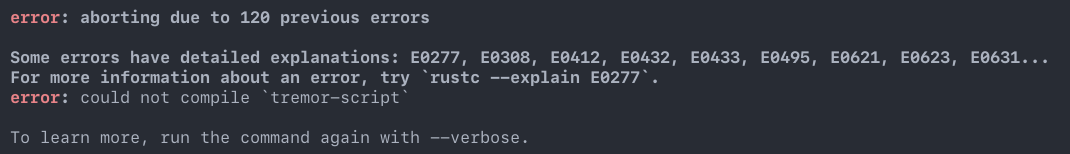
\includegraphics[width=\textwidth]{./Imagenes/errors.png}
    \caption{Al intentar evitar los tipos externos se produjeron más de 120
    errores de compilación.}%
    \label{fig:errors}
\end{figure}

\subsubsection{Encapsular el tipo externo}

Otra opción es crear un \emph{wrapper} para \code{halfbrown}, de la misma forma
que lo hace ya \abistable con otras librerías más conocidas. Este
encapsulamiento hace posible su uso desde el ABI de C de forma segura. Sin
embargo, estos ejemplos ya existentes son complejos~\cite{complexwrapper} y
difíciles de mantener, ya que tendrán que actualizarme con cada nueva versión de
\code{halfbrown}.

\subsubsection{Reimplementar el tipo con el ABI de C desde cero}

Similar a la solución anterior, pero con incluso más costoso, dado que también
requeriría reimplementar la funcionalidad. Puede parecer indeseable, pero es la
mejor forma de asegurar un rendimiento máximo. Los tipos externos mencionados
son parte de optimizaciones; encapsularlos podría tener un impacto en su
rendimiento y hacerlos inútiles.

Si esta parte del proyecto es lo suficientemente importante y existen los
recursos, debería considerarse. De hecho, el mismo tipo \code{Value} en Tremor
surgió por esta razón: ya existía \code{simd_json::Value} de otra librería, pero
carecía de la suficiente flexibilidad y el equipo implementó uno personalizado.

\subsubsection{Simplificar el tipo para la interfaz}

Esta última opción resultó ser la más sencilla de implementar: crear una copia
de \code{Value} cuyo único uso es para comunicarse entre runtime y plugins,
ilustrado en la Figura~\ref{fig:simplify}.

\begin{figure}
    \centering
    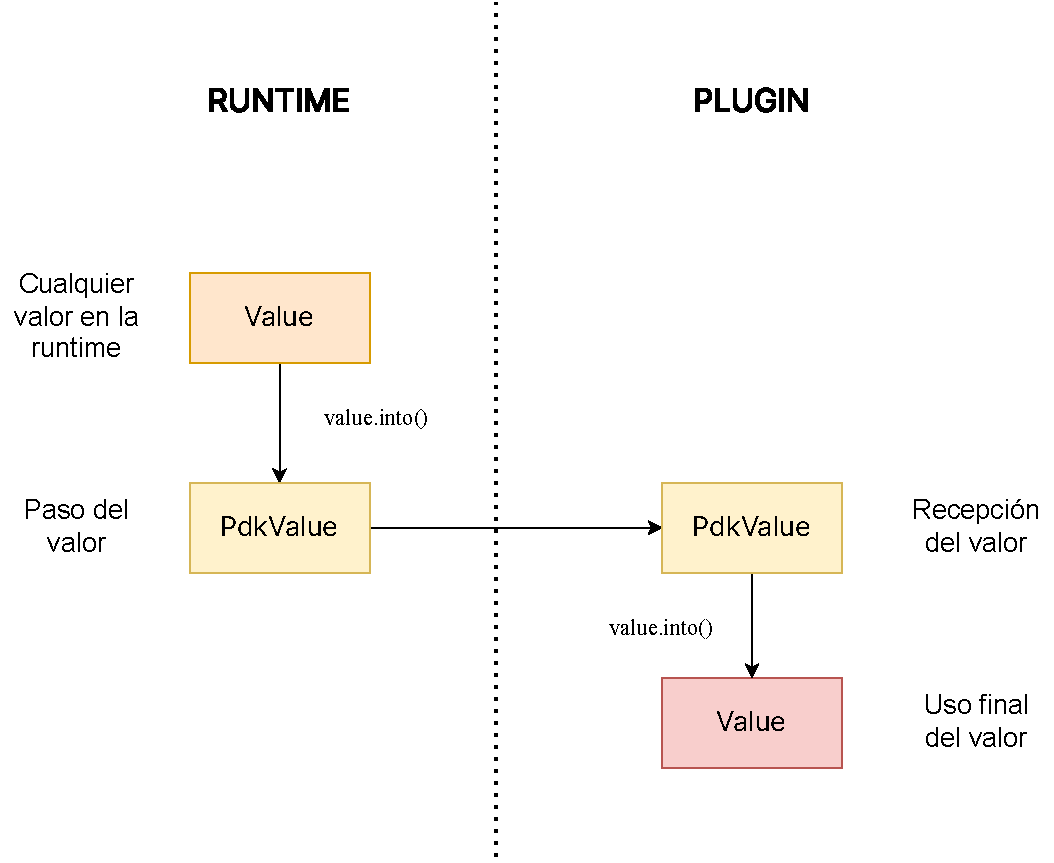
\includegraphics[width=10cm]{./Imagenes/simplify.pdf}
    \caption{Comunicación entre runtime y plugins en el PDK.}%
    \label{fig:simplify}
\end{figure}

Ya que es un tipo nuevo, no se romperá nada del código ya existente, y
únicamente hará falta cambiarlo donde se use la interfaz. Su implementación es
sencilla (notar el cambio de nombre a \code{PdkValue}):

\begin{minted}{rust}
pub enum PdkValue {
    /// Valores estáticos (enteros, booleanos, etc)
    Static(StaticNode),
    /// Tipo para cadenas de caracteres
    String(String),
    /// Tipo para listas
    Array(Vec<Value>),
    /// Tipo para objetos (mapas clave-valor)
    Object(Box<HashMap<String, PdkValue>>),
    /// Tipo para datos binarios
    Bytes(Vec<u8>),
}
\end{minted}

No es necesario escribir métodos adicionales para el nuevo \code{PdkValue}, solo
sus conversiones desde y hasta el tipo original, \code{Value}. Esto sería
equivalente a, en vez de pasar un \code{Vec<T>} al PDK, reemplzarlo con un
\code{*const u8} para los datos y un \code{u32} para la longitud. Simplemente
consiste en simplificar los tipos en la interfaz, y convertirlos de vuelta para
usar la funcionalidad completa.

El problema principal es que la conversión entre tipos es ahora $O(n)$ en vez de
$O(1)$, dado que es necesario iterar los datos en los objetos y vectores para la
conversión. Su uso sería el siguiente:

TODO: mejor si omito el código aquí con la conversión, no?

\begin{minted}{rust}
// Esta función es exportada por el plugin. Funcionará porque
// `PdkValue` está declarado con el ABI de C.
pub extern "C" fn plugin_funfuncue: PdkValue) {
    let value = Value::from(value);
    value.do_func()
}

// Esto se puede implementar en la runtime para facilitar su uso,
// convirtiendo al tipo original.
fn runtime_wrapper(value: Value) {
    plugin_func(value.into());
}
\end{minted}

Es la alternativa más sencilla, pero implica un coste de rendimiento; dos
conversiones implican iterar los datos dos veces. Tras mediciones posteriores,
se verificó que convertir los datos era un 5-10\% de la ejecución del programa.
Es menos de lo esperado, pero sigue sin ser suficiente para Tremor.

También tiene un coste de usabilidad; en comparación con tener un único
\code{Value}, es necesario convertir los tipos y posiblemente crear encapsularlo
con una función de más alto nivel (\code{runtime_wrapper}). Es una tarea
relativamente trivial, por lo que se podría automatizar con macros procedurales
en Rust, pero esto debería dejarse para el final del proyecto.

En conclusión, esta alternativa es la más fácil de implementar en el corto
plazo y por tanto la que mejor sigue \work. Una vez esté terminado, se puede
analizar el rendimiento y optar por una alternativa más eficiente, como
reescribir los tipos para el caso de uso específico de Tremor.

\subsection{Problemas con varianza y subtipado}

Otro problema muy importante 

\section{Separación de runtime e interfaz}

\section{Despliegue en producción}

\section{Lecciones aprendidas}

* Quizá incluir consejos de los mentores?

\begin{figure}
    \centering
    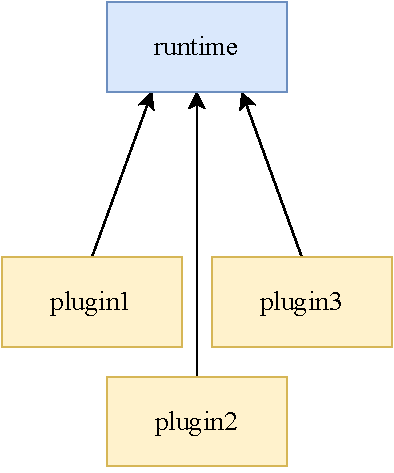
\includegraphics[width=6cm]{./Imagenes/separation-temporary.pdf}
    \caption{Ejemplo de uso de Tremor}%
    \label{fig:separation_temporary}
\end{figure}

\begin{figure}
    \centering
    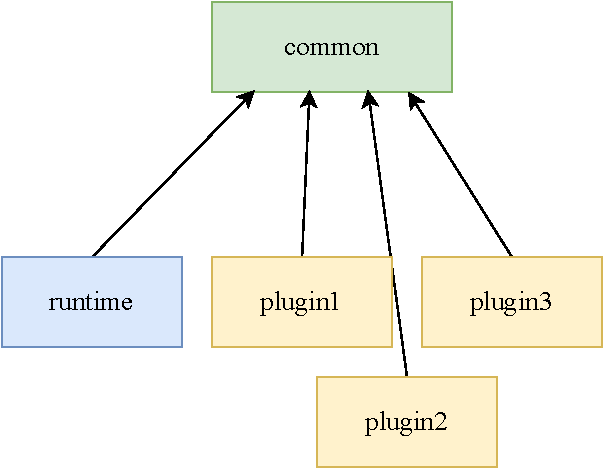
\includegraphics[width=7cm]{./Imagenes/separation.pdf}
    \caption{Ejemplo de uso de Tremor}%
    \label{fig:separation}
\end{figure}

\begin{figure}
    \centering
    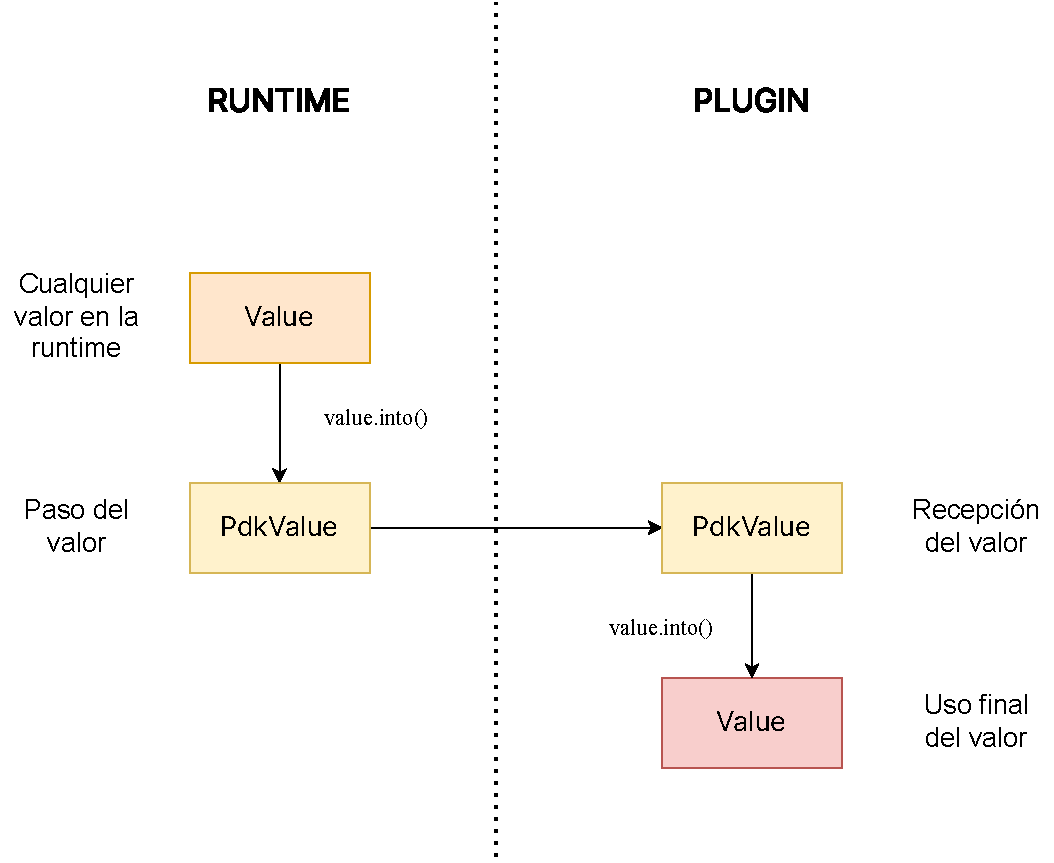
\includegraphics[width=\textwidth]{./Imagenes/simplify.pdf}
    \caption{Ejemplo de uso de Tremor}%
    \label{fig:simplify}
\end{figure}
